\chapter{Fetch Stage}

We are ready to build our fetch unit.  To do this, we will make one more unit, our instruction memory, then we will need to make a module to assemble all our units together.


\section{Instruction Memory}
The instructions are stored in memory, and are accessed by using the address where they are stored.  You can think of memory like a giant hotel for our data.  Each piece of data is stored in a room (memory location), which we can find by its room number (memory address).  To get a piece of data stored in memory (like an instruction) we need to take its address, go to that location, and grab the data.  A bunch of memory locations, accessed by an address is called an array.  Arrays in Verilog are declared like they are in C; the data type is specified, then the name, then the array size.  To store the instructions, we will need an array of 32-bit numbers (definitions.vh defines INSTR\_LEN as 32), which means the data type must be \verb2reg[`INSTR_LEN-1:0]2.  After the name is specified (mem in this case), we are going to use a parameter called SIZE to specify how big the array is: \verb2[SIZE-1:0]2.

The other interesting thing about this code is how to initialize the memory.  The default size of the memory is 1024 bytes, so we do not want to initialize this memory element by element in the code.  Fortunately Verilog gives you two functions to do this automatically: \$readmemb and \$readmemh.  The last letter specifies the base (binary or hexadecimal) of the data in the file.  White space separates fields, but the underscore character is ignored and thus can be used to make the values in a number more readable.  The readmemb function will be used to read the file `IMEMFILE and store the bits in the imem array.  This is done one time on initialization.  Then, you can access that data in imem at any time after that.  `IMEMFILE is defined in definitions.vh, and I provide this file, which contains 14 instructions.  However, you will need to update definitions.vh to point to your group's testfiles section rather than mine, or else it will not find the file.

\Verilog{Instruction Memory}{code:instmem}{../code/1_fetch/instr_mem.v}

The code is given in Listing~\ref{code:instmem}.  How will it be used?  What needs to be tested?  Consider those questions and write a testbench and verify it's operation.

\section{Fetch Stage}
Now we need to connect it together.  The components of our instruction fetch (sometimes called ifetch or just fetch) stage are shown in Figure~\ref{fig:fetch}.

\begin{wrapfigure}{L}{2in}
\caption{Instruction Fetch Stage.}\label{fig:fetch}
\begin{center}
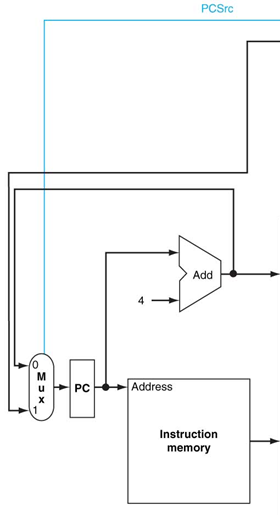
\includegraphics[width=2in]{../images/pipeline_fetch.png}
\end{center}
\end{wrapfigure}

Any wire (or reg) in the figure that comes in or goes out are input or output ports in the iFetch module.  In Figure~\ref{fig:fetch}, the blue wire is a control signal and comes ultimately from the control unit, which you will build in the decode stage.   Wires (or regs) that are completely contained in the figure are local to the iFetch module and are thus defined internally in the module.  The one exception to this is the current program counter (cur\_pc).  While there is no reason that it must be output from the iFetch module, I recommend making it an output so that it shows up on your simulation results, helping you to keep track of which instruction is currently executing.  

While the input and output signals are easily identified by the diagram, you must also determine the size of each signal and whether it is a wire or reg.  When you look at the figure I cut from a figure in the book, note that not every wire has a name.  If a wire is unlabeled, it is worth looking at other figures (like your text in chapter 4) to figure out what the signal is.  

IMPORTANT NOTE: Throughout your entire project, your signal names should follow the convention of the Freescale Semiconductor Verilog guide, which states that signal names should be all lower case, with words separated by an underscore.   

Once you have figured out all your connecting signals (wires and regs), you should identify the components you are going to use.  We have already created the modules, so now we just need to tell Verilog to instantiate them (build one) in the iFetch module.  Again choose your names wisely.  I have instantiated them for you in Listing~\ref{code:fetch}, but I haven't made the connections yet.  You must use knowledge gained from the wiring diagram to hook the components together with the available wires.  You should not need to create any more wires and registers.  It is just a matter of connecting the components together correctly.

The code, minus the connections, is listed below in Listing~\ref{code:fetch}.    

\Verilog{Starter code for the fetch stage.}{code:fetch}{../code/1_fetch/iFetch.v}

\section{Fetch Testbench}
Once you have made your connections, you should test the operation of the iFetch module by creating iFetch\_test.v.  You know you checked your individual modules, but there could be errors, or unexpected behavior when you put them together.  Sometimes weird timings between modules causes signals to be missed and such.  

Your testbench should set the inputs into the iFetch stage and verify that the correct outputs are produced. You should test both sequential operation (PC incrementing by 4) and branching.  When you test branching, keep in mind that my provided instruction file (instrData.data) only contains 14 instructions, so don't branch beyond the end of the file.

As we progress through this lab, you will learn how critical timing is.  Please look at the cur\_pc value and the instruction value and verify that the instruction that was fetched is the correct instruction, according to instrData.data and the current program counter.  Make sure to switch back and forth between sequential and branching to make sure that this works properly, 

\section{Lab Writeup}
For the Lab 3 report, only describe iFetch.v, iFetch\_test.v, and instr\_mem\_test.v.  You have already described the other files, except instr\_mem.v, which I provided.  iFetch.v is all about the module connections and how the modules interact with each other.  Focus the Interface, Design, and Implementation parts of your lab report on that aspect.  Then describe iFetch\_test.v, and instr\_mem\_test.v in the Test Bench Design section, and show the results for both.


\section{Your Assignment}
You are to:
\begin{enumerate}
\item Write a testbench for the memory in Listing~\ref{code:instmem}.
\item Finish the fetch stage and write a testbench to verify it.
\item Run the simulations and generate a timing diagrams.
\item  Write up a lab report in \LaTeX\ following the lab format in \verb1LabN.tex1 and generate a pdf file.
\item Upload the pdf and all the Verilog files to Canvas.
\end{enumerate} 